\begin{figure}[H]
    \centering
    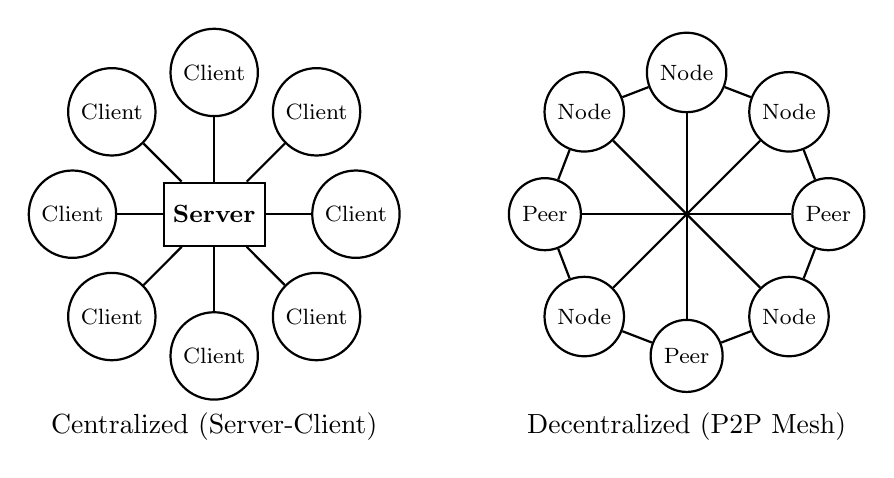
\begin{tikzpicture}[
        clientNode/.style={
            circle,
            draw,
            thick,
            minimum size=0.8cm,
            font=\footnotesize
        },
        serverNode/.style={
            rectangle,
            draw,
            thick,
            minimum size=0.8cm,
            font=\small\bfseries
        },
        line/.style={
            thick
        }
    ]
        \node[serverNode] (server) at (0,2) {Server};
        
        \node[clientNode] (c1) at (0,3.8)  {Client};
        \node[clientNode] (c2) at (1.3,3.3) {Client};
        \node[clientNode] (c3) at (1.8,2)   {Client};
        \node[clientNode] (c4) at (1.3,0.7) {Client};
        \node[clientNode] (c5) at (0,0.2)  {Client};
        \node[clientNode] (c6) at (-1.3,0.7){Client};
        \node[clientNode] (c7) at (-1.8,2)  {Client};
        \node[clientNode] (c8) at (-1.3,3.3){Client};
        
        \draw[line] (server) -- (c1);
        \draw[line] (server) -- (c2);
        \draw[line] (server) -- (c3);
        \draw[line] (server) -- (c4);
        \draw[line] (server) -- (c5);
        \draw[line] (server) -- (c6);
        \draw[line] (server) -- (c7);
        \draw[line] (server) -- (c8);
        
        \node[anchor=north, yshift=-0.4cm] at (0,0) {Centralized (Server-Client)};

        \node[clientNode] (p1) at (6,3.8)  {Node};
        \node[clientNode] (p2) at (7.3,3.3) {Node};
        \node[clientNode] (p3) at (7.8,2)   {Peer};
        \node[clientNode] (p4) at (7.3,0.7) {Node};
        \node[clientNode] (p5) at (6,0.2)  {Peer};
        \node[clientNode] (p6) at (4.7,0.7) {Node};
        \node[clientNode] (p7) at (4.2,2)   {Peer};
        \node[clientNode] (p8) at (4.7,3.3) {Node};
        
        \draw[line] (p1) -- (p2);
        \draw[line] (p2) -- (p3);
        \draw[line] (p3) -- (p4);
        \draw[line] (p4) -- (p5);
        \draw[line] (p5) -- (p6);
        \draw[line] (p6) -- (p7);
        \draw[line] (p7) -- (p8);
        \draw[line] (p8) -- (p1);

        \draw[line] (p1) -- (p5);
        \draw[line] (p3) -- (p7);
        \draw[line] (p2) -- (p6);
        \draw[line] (p4) -- (p8);
        
        \node[anchor=north, yshift=-0.4cm] at (6,0) {Decentralized (P2P Mesh)};

    \end{tikzpicture}
    \vspace{0.3cm}
    \caption{Centralized (Server-Client) and Decentralized (Peer-to-Peer) network}
    \label{fig:comparison_topologies}
\end{figure}